\input{preamble}
\usepackage[backend=biber, style=gost-numeric, sorting=none]{biblatex}
\usepackage{subfigure}

\addbibresource{references.bib}

\theoremstyle{definition}
\newtheorem*{definition}{Определение}
\theoremstyle{plain}
\newtheorem{lemma}{Лемма}
\newtheorem{theorem}{Теорема}
\newtheorem{assumption}{Предположение}



%  межсточный интервал
\linespread{1.5}
% абзацный интервал
\setlength{\parindent}{1.25cm}

\setcounter{page}{2}

\title{Сходимость с оценкой вероятностей больших отклонений для задач выпуклой оптимизации и седловых задач в условиях повышенной гладкости}

\date{}

\begin{document}
	
	%\maketitle
	\hspace{0pt}
	\vfill
	\begin{center}
		\tableofcontents
	\end{center}
	\vfill
	\hspace{0pt}
	
	\newpage
	
	\hspace{0pt}
	\vfill
	
	\begin{abstract}
		
		Классические результаты стохастической оптимизации, как правило, формулируются в терминах числа итераций, необходимых для достижения $\varepsilon$-точности по математическому ожиданию функции. В данной работе разрабатывается обёртка над алгоритмами сходимости по математическому ожиданию, обеспечивающая гарантию сходимости с высокой вероятностью для задач выпуклой оптимизации и седловых задач, причем за эффективную сложность и для функций различной степени гладкости и выпуклости. Полученные гарантии сходимости подтверждаются на вычислительных экспериментах.
		
	\end{abstract}
	
	\textbf{Ключевые слова}: {\small стохастическая выпуклая оптимизация, стохастические седловые задачи, сходимость с высокой вероятностью, оценка вероятности больших отклонений, проксимальный метод, неравенства концентрации}.
	
	\vfill
	\hspace{0pt}
	
	\newpage
	
	
	\section{Введение}\label{Intro}
	
	В данной работе рассматривается задача стохастической оптимизации 
    \begin{equation} \label{min_problem}
    \min_{x \in \R^d} f(x) := \E_{\xi}{f(x, \xi)},  
    \end{equation}
     где случайная величина $\xi$ из фиксированного, но неизвестного распределения $\mathcal{P}$: $\xi \sim \mathcal{P}$. 
     
     Как правило, результатом стохастических градиентных методов является точка $x_{\e}$ такая, что 
    \begin{equation} \label{expectation_conv}
   \E{f(x_{\e})} - \min f \le \e.  
    \end{equation}
Такую сходимость в дальнейшем будем называть сходимостью <<по математическому ожиданию>>. Стоимость таких алгоритмов, например, стохастического градиентного спуска (Stochastic Gradient Descent, SGD) в терминах количества вызовов стохастического градиентного оракула $\mathcal{O} (\frac{1}{\e^2})$ в выпуклом случае и $\mathcal{O} (\frac{1}{\e})$ в сильно выпуклом случае (см. \cite{nemirovskij1983problem}, \cite{polyak1992acceleration}, \cite{ghadimi2013optimal}, \cite{hazan2014beyond}).

В данной работе мы рассматриваем алгоритмы, результатом которых являются точки $x_{\e, p}$, удовлетворяющие условию
\begin{equation} \label{high_prob_conv}
   \mathds{P} (f(x_{\e, p})-\min f \le \e) \ge 1 - p,  
\end{equation}
где число $p > 0$ может быть достаточно маленьким. Проще говоря, мы ищем такие решения, для которых вероятность того, что невязка меньше желаемой точности $\e$ достаточно большая. Здесь под невязкой будет пониматься разность значений функции в точке и минимума этой функции. Формулу \eqref{high_prob_conv} можно переписать в другом виде:
\begin{equation} \label{deviation_prob}
   \mathds{P} (f(x_{\e, p})-\min f \ge \e) \le p,  
\end{equation}
Формулу \eqref{high_prob_conv} можно интерпретировать как сходимость <<с высокой вероятностью>>, а формулу \eqref{deviation_prob} как оценку вероятности больших отклонений, что отражено в названии дипломной работы.
Из неравенства Маркова ясно, что \eqref{high_prob_conv} или \eqref{deviation_prob} можно гарантировать, если найти точку $x_{\e, p}$ такую, что $\E{f(x_{\e, p})} - \min f \le p\e$. Однако для этого необходимо $\mathcal{O} (\frac{1}{p^2\e^2})$ или $\mathcal{O} (\frac{1}{p\e})$ вызовов стохастического оракула, то есть сложность существенно возрастает при малых $p$. Существует несколько статей, в которых сложность относительно $p$ снижается до логарифмической $\log(\frac{1}{p})$, однако либо в то же время ухудшается сложность относительно $\e$ (\cite{bousquet2002stability}, \cite{nesterov2008confidence}, \cite{shalev2009stochastic}), либо делаются более жесткие ограничения на шум стохастического градиента (\cite{nemirovski2009robust}, \cite{juditsky2014deterministic}, \cite{ghadimi2012optimal}, \cite{ghadimi2013optimal}, \cite{harvey2019simple}, \cite{harvey2019tight}): он предполагается субгауссовским, то есть имеющим <<легкие хвосты>>. Техника клиппирования (см.\cite{gorbunov2020stochastic}, \cite{gorbunov2024high}) хоть и позволяет работать с <<тяжелыми хвостами>> шума стохастического градиента, но требует исследования теоретических гарантий для каждого нового алгоритма,то есть не является общей оболочкой над алгоритмами.

В работе \cite{davis2021low} был разработан общий алгоритм, работающий и в случае <<тяжелых хвостов>> распределения шума стохастического градиента, при этом требующий не очень большого числа вызовов оракула.  В этой работе рассматривается оракул $\mathcal{M}(f, \e)$, возвращающий точку $x_{\e}$ такую, что $\mathds{P} (f(x_{\e})-\min f \le \e) \ge \frac{2}{3}$. В частности, такой оракул может быть порожден любым алгоритмом стохастической оптимизации, возвращающим точку $x_{\e}$ такую, что $\E{f(x_{\e})} - \min f \le \frac{\e}{3}$ (следствие неравенства Маркова).  Авторы показали, что для $\mu$-сильно выпуклых $L$-гладких функций алгоритм, решающий задачу \eqref{high_prob_conv} требует $\log({\frac{\log{\kappa}}{p}})\log{\kappa}\cdot \mathcal{C}_{\mathcal{M}}(f, \frac{\e}{\log{\kappa}})$ вызовов стохастического оракула, где  $\mathcal{C}_{\mathcal{M}}(f, \e)$ - стоимость (сложность) вызова такого оракула. Таким образом, задача сходимости с высокой вероятностью сложнее (в смысле оракульной сложности) задачи сходимости по матожиданию лишь в логарфимическое по $\frac{1}{p}$ и полилогарифмическое по числу обусловленности $\kappa := \frac{L}{\mu}$ раз. 

В данной дипломной работе результаты работы \cite{davis2021low} обобщаются на негладкий и не сильно выпуклый случаи. Сложность остается логарифмической по $\frac{1}{p}$, однако ухудшается сложность относительно $\e$, но лишь логарифмически. Таким образом, здесь существующая обертка над алгоритмами адаптирована для более широких классов минимизируемых функций. 

В последней части работы мы также решаем выпукло-вогнутые седловые задачи 
\begin{equation} \label{saddle problem}
    \min_{x \in X} \max_{y \in Y} \Phi (x, y) := \E{\Phi_{\xi}(x, y)}
\end{equation}
 являющиеся актуальными, в частности, в связи с  развитием обучения с подкреплением (reinforcement learning; см., например, \cite{puterman2014markov}, \cite{wang2017primal}). Так же, как и в задачах выпуклой оптимизации, в большинстве работ решаются задачи сходимости по математическому ожиданию функций (\cite{nemirovski2009robust}, \cite{shalev2013stochastic}, \cite{zhang2017stochastic}, \cite{yan2019stochastic}, \cite{zhang2021generalization}) $$\mathbb{E}[\Delta_\Phi(\hat x,\hat y)]\leq \epsilon\qquad\mbox{или}\qquad \mathbb{E}[\Delta_\Phi^w(\hat x,\hat y)]\leq \epsilon.$$. Здесь для любых $(\hat x,\hat y)\in\mathcal{X}\times\mathcal{Y}$ введен зазор двойственности 
\begin{equation}\label{gap}
    \Delta_{\Phi}(\hat{x},\hat{y}):=\max_{y\in\mathcal{Y}} \Phi(\hat{x},y)-\min_{x\in\mathcal{X}} \Phi(x,\hat{y}) =: f(\hat{x}) - g(\hat{y}).
\end{equation} 
и его слабая версия
\begin{equation} \label{weak_gap}
    \Delta^w_{\Phi}(\hat{x},\hat{y}):=\Phi(\hat{x},y^*)-\Phi(x^*,\hat{y}),
\end{equation}
где $(x^*, y^*)$ - решение задачи \eqref{saddle problem}.
Целью данного исследования является поиск таких решений, что 

\begin{equation}
    \mathbb{P}\left[\Delta_{\Phi}(\bar x,\bar y) \leq \epsilon \right] \geq 1-p 
    \label{equ: high prob guarantee}
\end{equation}

На базе методов, предложенных в статье \cite{davis2021low} для задач выпуклой оптимизации в статье \cite{li2024general} строятся (по аналогии) методы для выпукло-вогнутых седловых задач с обеспечением гарантий сходимости высокой вероятности за небольшую сложность. Так как решение седловых задач можно рассматривать, обобщая результаты для задач минимизации (\cite{воронцова2021выпуклая}), начнем с подробного рассмотрения последних.

\section{Постановка задачи}
Пусть $\R^d$ - евклидово пространство со скалярным произведением $\langle \cdot, \cdot \rangle$ и индуцированным им нормой $\|x\|_2 = \langle x, x\rangle, x \in \R^d$. Всюду далее под $\|\cdot\|$ подразумевается евклидова норма. Замкнутый шар с центром в точке $x$ и радиусом $\e$ будем обозначать $B_{\e} (x)$. 

Будем решать задачу стохастической оптимизации
    \begin{equation} \label{min_problem}
    \min_{x \in \R^d} f(x) := \E{f(x, \xi)}.  
    \end{equation}
при следующих предположениях на функцию $f(x)$:

\begin{assumption} \label{ass:convex}
    Исследуемая функция $f:\R^d \to \R$ $\mu$-сильно выпуклая, то есть $\forall x, y$ выполнено:
    \begin{equation} \label{convex}
        f(y) \ge f(x) + \langle \nabla f(x), y - x \rangle + \frac{\mu}{2} ||y - x||^2
    \end{equation}
\end{assumption}

\begin{assumption}\label{ass:smooth}
    Функция $f: \R^d \to \R$  -  $(L, \gamma)$-гладкая, то есть $\forall x, y \in B_{R} (x^*), \  R = \|x_0 - x^*\|\}$ выполнено:
\begin{equation} \label{smooth}
f(y) \leq f(x) + \langle \nabla f(x), y - x \rangle + \frac{L}{2}\|y - x\|^2 + \gamma
\end{equation}
где $\nabla f(x) \in \partial f(x)$ - произвольный субградиент функции $f$ в точке $x$.
\end{assumption}

\begin{assumption} \label{ass: Holder}
    Градиент функции $f(x)$ удовлетворяет условию Гёльдера, то есть $\exists \nu \in [0, 1]$ такое, что $\forall x, y \in B_{R} (x^*) $ имеет место неравенство

    \begin{equation} \label{Holder}
        \|\nabla f(y) - \nabla f(x)\| \le L_{\nu} \|y - x\|_2^{\nu}, \ L_0 < \infty
    \end{equation}   
\end{assumption}

Заметим, что при $\nu = 1$ предположение \ref{ass: Holder} является просто условием $L_1-$гладкости. При $\nu = 0$ же предположение \ref{ass: Holder} является условием $L_0-$липшицевости. Далее будем обозначать $L_1 = L$ и $L_0 = M$.

Предположение \eqref{ass:smooth} введено для того, чтобы  смотреть на гладкий и негладкий случаи единообразно. Действительно, при $\gamma = 0$ это и есть условие гладкости. Если же функция негладкая, но $M-$липшицева ($\|\nabla f(y) - \nabla f(x)\| \le M$), то неравенство \eqref{smooth} всё равно будет выполняться при $L = \frac{M^2}{2\gamma}$. Доказательство этого утверждения можно найти в \cite{nesterov2015universal}.

\begin{lemma} \label{lemma:nesterov}
    Если для градиента функции $f(x)$ выполнено условие Гёльдера \eqref{Holder}, то такая функция $(L, \gamma)$-гладкая (см. \eqref{smooth}) при $$L = L_{\nu} \left(\frac{L_{\nu}}{2 \gamma} \frac{1-\nu}{1+\nu}\right) ^{\frac{1-\nu}{1+\nu}}.$$
    В частности, при $\nu = 0$ $L = \frac{M^2}{2\gamma}$.
\end{lemma}

Напомню, что эта работа сосредоточена на эффективном решении задачи оптимизации со следующей мерой качества \eqref{high_prob_conv}:
\begin{equation*} 
   \mathds{P} (f(x_{\e, p})-\min f \le \e) \ge 1 - p,  
\end{equation*}

При дальнейшем изложении нам будет важно, сохраняется ли <<слабая гладкость>> (предположение \ref{ass:smooth}) при добавлении регуляризационного слагаемого $\frac{\lambda}{2} \|x - z\|^2$, где $z$ - некоторая фиксированная точка. На этот вопрос отвечает следующая лемма.

\begin{lemma} \label{lemma:regular_smooth}
    Пусть функция $f(x)$ - $(L, \gamma)$-гладкая. Тогда функция $h(x) = f(x) + \frac{\lambda}{2} \|x - z\|^2$ является $(L + \lambda, \gamma)$-гладкой.
\end{lemma}
\begin{proof}
    Действительно, так как функция $f(x)$ - $(L, \gamma)$-гладкая, то
    \[f(y) \leq f(x) + \langle \nabla f(x), y - x \rangle + \frac{L}{2}\|y - x\|^2 + \gamma.\] 
    Это эквивалентно
    \[h(y) - \frac{\lambda}{2} \|y - z\|^2 \leq h(x) - \frac{\lambda}{2} \|x - z\|^2 + \langle \nabla h(x) - \lambda (x - z), y - x \rangle + \frac{L}{2}\|y - x\|^2 + \gamma\] или
    \[h(y) \leq h(x) + \langle \nabla h(x), y - x \rangle + \frac{L}{2}\|y - x\|^2 + \frac{\lambda}{2} \|y - z\|^2 - \frac{\lambda}{2} \|x - z\|^2  - \lambda \langle x - z, y - x \rangle+ \gamma\]
    В силу того, что $\frac{\lambda}{2} \|y - z\|^2 - \frac{\lambda}{2} \|x - z\|^2  - \lambda \langle x - z, y - x \rangle = \frac{\lambda}{2} \|y - x\|^2$
    получаем $(L + \lambda, \gamma)$-гладкость функции $h(x) = f(x) + \frac{\lambda}{2} \|x - z\|^2$ по определению:
    \[h(y) \leq h(x) + \langle \nabla h(x), y - x \rangle + \frac{L + \lambda}{2}\|y - x\|^2 + \gamma\]
    
    
\end{proof}

\section{Техники и алгоритмы}

Далее описываемая оболочка над алгоритмами сходимости по математическому ожиданию для обеспечения сходимости с высокой вероятностью зиждется на двух методах: RDE (Robust Distance Estimation, робастная оценка расстояний) и проксимальный метод.

\subsection{Robust distance estimation}

Пусть исследуемая функция $f:\R^d \to \R$ $\mu$-сильно выпуклая (т.е. $f(x)-\frac{\mu}{2}||x||^2$ - выпуклая) и $L$-гладкая (т.е. дифференцируемая с $L$-липшицевым градиентом). Для такой функции для всех точек $x, y \in \R^d$ справедливо:
\[\langle \nabla f(x), y - x \rangle + \frac{\mu}{2} ||y - x||^2 \le f(y) - f(x) \le \langle \nabla f(x), y - x\rangle + \frac{L}{2} ||y - x||^2.\]
Для точки $x^*$, в которой достигается минимум функции $f$ тогда справедливо (с учетом необходимого условия $\nabla f(x^*) = 0$):
\[\frac{\mu}{2} ||x- x^*||^2 \le f(x) - f(x^*) \le \frac{L}{2} ||x - x^*||^2\]
Отмечу, что в дальнейшем будет полезно более общее неравенство для $(L, \gamma)$-гладких функций:
\begin{equation} \label{approx_smooth}
    f(x) - f(x^*) \le \frac{L}{2} ||x - x^*||^2 + \gamma
\end{equation}
Далее $\min f = f(x^*) =: f^*$.

Обозначим за $\mathcal{D}(\e)$  - оракул, возвращающий точку $\mathds{P}[||x-x^*|| \le \e] \ge \frac23$. Можно сделать $m$ вызовов этого оракула $x_1, ..., x_m$ и выбрать среди полученных точек такую $x_{i^*}$, вокруг которой класстеризуются остальные точки.

\begin{algorithm}[H]
	{\bf Вход:}  доступ к оракулу $\mathcal{D}(\e)$ и число его вызовов $m$. \\
	Вызываем  оракул $\mathcal{D}(\e)$ $m$ раз. Обозначим множество его ответов за  $X=\{x_1,\ldots, x_m\}$.
	
	{\bf В цикле } $i=1,\ldots,m$:
    
	\hspace{20pt} Вычисляем $r_i=\min\{r\geq 0: |B_{r}(x_i)\cap X|>\frac{m}{2}\}$.
	
	 Устанавливаем $i^*=\argmin_{i\in [1,m]} r_i$ 

	 {\bf Возвращаем} $x_{i^*}$		\\
	\caption{Robust Distance Estimation (RDE) $\mathcal{D}(\varepsilon,m)$	%: PSSM($x_0,T,\{\alpha_t\}$)
	}
	\label{alg:rde}
\end{algorithm}


%\begin{center}
%   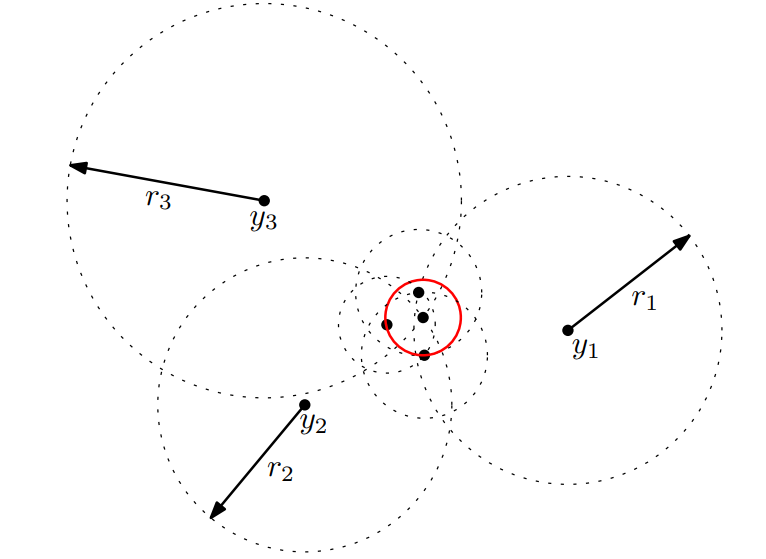
\includegraphics[width=5cm, height=4cm]{RDE.png} 
%\end{center}

\begin{theorem} \label{th:rde}
Точка $x_{i^*}$, возвращаемая алгоритмом RDE, удовлетворяет условию
\[\mathds{P} (||x_{i^*} - x^*|| \le 3 \e) \ge 1 - e^{-\frac{m}{18}}\]
\end{theorem}

Доказательство теоремы основано на неравенствах концентрации, его можно найти в \cite{nemirovskij1983problem} или в \cite{hsu2016loss}.

Опишем, как алгоритм RDE \ref{alg:rde} может обеспечивать сходимость с высокой вероятностью.
Пусть точки $x_i$ ($i = 1, ..., m$) таковы, что $\E{f(x_{\e})} - \min f \le \frac{\e}{3}$, то есть могут быть сгенерированы алгоритмом сходимости по мат. ожиданию.  По неравенству Маркова тогда автоматически следует, что $\mathds{P} (f(x_i) - f^* \le \e ) \ge \frac{2}{3}$. Из $\mu$-сильной выпуклости получаем $\mathds{P} (||x_i - x^*|| < \sqrt{\frac{2 \e}{\mu}} =: \delta) \ge \frac{2}{3}$. Применив к этим точкам алгоритм RDE (\ref{alg:rde}), получим точку $x_{i^*}$, удовлетворяющую неравенству $\mathds{P}(||x_{i^*} - x^*|| < 3 \delta) \ge 1 - e^{-\frac{m}{18}}$. Из $L$-гладкости функции $f$ тогда следует, что $\mathds{P}(f(x_{i^*}) - f^* \le \frac{L}{2}(3\delta)^2 = 9 \frac{L}{\mu}\e) \ge 1 - e^{-\frac{m}{18}}$. Таким образом, генерируя точки алгоритмом, дающим гарантии сходимости с точностью $\e$ по матожиданию, но не с высокой вероятностью, RDE обеспечивает гарантию сходимости с высокой вероятностью, но лишь с $\kappa \e$-точностью, где число обусловленности $\kappa = \frac{L}{\mu} \gg 1$ может быть достаточно большим. Для нивелирования этой проблемы в статье \cite{davis2021low} был предложена процедура $proxBoost$, которая будет описана далее. На процедуру RDE можно посмотреть и под другим углом. Желаемое качество сходимости \eqref{high_prob_conv} обеспечивается, если $m \sim \ln{\frac{1}{p}}$ раз вызвать оракул $\mathcal{M}(f, \frac{\e}{\kappa})$, что требует итоговой оракульной сложности $\mathcal{O}\left(\log{\frac{1}{p}} \cdot \mathcal{C}_{\mathcal{M}}(f, \frac{\e}{\kappa}) \right)$, в которой содержится нежелаемый множитель $\kappa$. Предлагаемый в \cite{davis2021low}
подход уменьшает сложность по числу обусловленности $\kappa$ до логарифмического.
\subsection{Проксимальный метод}
Зафиксируем возрастающую последовательность $\lambda_0, ..., \lambda_T$ и последовательность точек $x_0, ..., x_T$. Для каждого $i = 0, ..., T$ введем функцию 
\[f^i(x):=f(x) + \frac{\lambda_i}{2}||x - x_i||^2\]
\[\bar{x}_{i + 1} := \argmin_x f^i (x)\]

В качестве $x_i$ можно брать $x_i = \bar{x}_i$ для $i \ge 1$. Так как точное вычисление точки минимума чаще всего невозможно, будем следить лишь за $||\bar{x}_i - x_i||$. Для простоты, $\bar{x}_0 := \argmin f$, $\lambda_{-1} := 0$.

\begin{theorem} \label{th: proximal}
    (Неточный проксимальный метод) Для всех $j \ge 0$ выполняется следующее неравенство:
    \[f^j(\bar{x}_{j + 1}) - f^* \le \sum_{i = 0}^{j}\frac{\lambda_j}{2}||\bar{x}_i - x_i||^2.\]
    Слндовательно, имеем декомпозицию функциональной ошибки:
    \[f(x_{j + 1}) - f^* \le (f^j(x_{j + 1}) - f^j(\bar{x}_{j + 1})) + \sum_{i = 0}^{j}\frac{\lambda_j}{2}||\bar{x}_i - x_i||^2.\]
    Если функция $f$ еще и $(L, \gamma)$-гладкая, то для всех $j \ge 0$ выполнена оценка:
    \begin{equation} \label{decomposition}
        f(x_j) - f^* \le \frac{L + \lambda_{j - 1}}{2} ||\bar{x}_j - x_j||^2 + \gamma + \sum_{i = 0}^{j - 1}\frac{\lambda_j}{2}||\bar{x}_i - x_i||^2.
    \end{equation}
\end{theorem}

Основным результатом Теоремы \eqref{th: proximal} является декомпозиция функциональной ошибки на ошибку на последнем шаге $(f^T(x_{j + 1}) - f^T(\bar{x}_{j + 1}))$ и накопленную ошибку $\sum_{i = 0}^{T}\frac{\lambda_j}{2}||\bar{x}_i - x_i||^2$. Доказательство можно найти в \cite{davis2021low}. Последний пункт теоремы следует непосредственно из леммы \ref{lemma:regular_smooth}. Для достаточно больших $T$ можно гарантировать то, что функция $f^T$ хорошо обусловлена. Использование преимуществ результатов теорем \eqref{th:rde} и \eqref{th: proximal} навело авторов \cite{davis2021low} разработку алгоритм $proxBoost$, который здесь представлен в обобщенном виде для $(L, \gamma)$-гладких функций.

\begin{algorithm}[H]
    {\bf Вход:} $\delta\geq 0$, $p\in (0,1)$, $T\in \mathbb{N}$\\
	Установить $\lambda_{-1}=0$, $\varepsilon_{-1}=\sqrt{\frac{2\delta}{\mu}}$
	
	Получить точку $x_{0}$, удовлетворяющую $\|x_{0}-\bar x_0\|\leq \varepsilon_{-1}$ с вероятностью $1-p$.
	
	{\bf В цикле }{$j=0,\ldots,T-1$}{
    
	  \hspace{20pt} Установить $\varepsilon_{j}=\sqrt{\frac{2\delta}{\mu+\lambda_{j}}}$
	
	\hspace{20pt} 
	Получить точку $x_{j+1}$, удовлетворяющую
	\begin{equation}\label{eqn:keyesneededblah}
	\PP\left[\|x_{j+1}-\bar x_{j+1}\|\leq \varepsilon_{j} \mid E_{j}\right]\geq 1-p,
	\end{equation}
	\hspace{20pt} 
	где $E_j$ обозначает событие $E_j:=\left\{x_i\in B_{\varepsilon_{i-1}}(\bar x_i)\textrm{ for all }i\in [0,j]\right\}$.}

\smallskip
Получить точку $x_{T+1}$, удовлетворяющую
	\begin{equation}\label{eqn:clean_up}
	\PP\left[f^{T}(x_{T+1})-\min f^{T}\leq \delta \mid E_{T}\right]\geq 1-p.
	\end{equation}
	
	{\bf Выход:} $x_{T+1}$
	
	
	\caption{$\cb(\delta, p, T)$	%: PSSM($x_0,T,\{\alpha_t\}$)
	}
	\label{alg: proxBoost}
\end{algorithm}

\begin{theorem}[О proxBoost]\label{thm:conf_boost_basic}
Зафиксируем константу $\delta>0$, вероятность отказа $p\in (0,1)$ и натуральное число $T\in \mathbb{N}$.
Тогда с вероятностью не менее $1-(T+2)p$, точка $x_{T+1}=\cb(\delta,p,T)$ удовлетворяет
	\begin{equation}\label{eqn:gap_bounds}
	f(x_{T+1})-\min f \leq \delta \left(1+ \sum_{i=0}^T \frac{\lambda_i}{\mu+\lambda_{i-1}}\right).
	\end{equation}
\end{theorem}
\begin{proof}
Сначала докажем по индукции оценку
\begin{equation}\label{eqn:induct_prob}
\PP[E_t]\geq 1-(t+1)p\qquad \textrm{для всех }t=0,\ldots, T.
\end{equation}
База индукции $t=0$ следует непосредственно из определения $x_0$.
Теперь предположим, что \eqref{eqn:induct_prob} выполняется для некоторого индекса $t-1$.
Тогда из предположения индукции и определения $x_t$ следует
$$\PP[E_t]= \PP[E_{t}\bigl\vert E_{t-1}]\PP[E_{t-1}]\geq \left(1-p\right)\left(1-tp\right)\geq 1-(t+1)p,$$
что завершает шаг индукции. Таким образом, неравенства \eqref{eqn:induct_prob} выполняются. Определим событие $$F=\{f^{T}(x_{T+1})-\min f^T\leq \delta\}.$$
Тогда
$$\PP[F\cap E_T]=\PP[F\mid E_T]\cdot \PP[E_T]\geq (1-(T+1)p)(1-p)\geq 1-(T+2)p.$$
Теперь предположим, что выполнено событие $F\cap E_{T}$. Тогда
\begin{equation*}
f(x_{T+1})-\min f\leq (f^{T}(x_{T+1})-f^{T}(\bar x_{T+1}))+\sum_{i=0}^{T} \frac{\lambda_i}{2}\|\bar x_{i}-x_{i}\|^2\leq \delta+\sum_{i=0}^T \frac{\delta\lambda_i}{\mu+\lambda_{i-1}},
\end{equation*}
где последнее неравенство использует определения $x_{T+1}$ и $\varepsilon_j$. Это завершает доказательство.
\end{proof}


Отметим, что данная теорема не использует свойства гладкости или негладкости функции. Глядя на оценку~\eqref{eqn:gap_bounds}, мы видим, что итоговая ошибка $f(x_{T+1})-\min f$ контролируется суммой $\sum_{i=0}^T \frac{\lambda_i}{\mu+\lambda_{i-1}}$. Если выбрать проксимальные параметры геометрически возрастающими $\lambda_i=\mu 2^i$, то в этом случае каждый член суммы $\frac{\lambda_{i}}{\mu+\lambda_{i-1}}$ ограничен сверху двойкой. Более того, если $f$ является $L$-гладкой, то число обусловленности $\frac{L+\lambda_T}{\mu+\lambda_T}$ для функции $f^T$ оказывается ограничено двойкой уже после $T=\lceil\log(L/\mu)\rceil$ итераций.

\section{Основной алгоритм}\label{sec:conseq_approx}
Часто сложность стохастических градиентных методов, то есть количество оракульных вызовов, необходимых для достижения желаемой точности $\EE [f(x_i)]-f^*\leq \delta$ зависит от начальной невязки $f(x_0)-f^*$. Так что мы должны иметь доступ к верхней оценке этой невязки $\Delta : \Delta\geq f(x_0)-f^*$. В предложенном далее алгоритме мы будем динамически обновлять соответствующие верхние оценки.

\begin{assumption}\label{ass:alg_min_orc}{\em
Введем вспомогательную проксимальную задачу
$$\min_y~ \varphi_x(y):=f(y)+\frac{\lambda}{2}\|y- x\|^2,$$
Пусть $\Delta>0$ такое, что $\varphi_x(x)-\min \varphi_x\leq \Delta$.
Будем обозначать $\alg(\delta,\lambda,\Delta, x)$ процедуру (оракул), которая возвращает точку $y$ такую, что
$$\PP(\varphi_x(y)-\min \varphi_x\leq \delta)\geq\frac{2}{3}.$$}
\end{assumption}

Так как функция $\varphi_x$ $(\mu+\lambda)$-сильно выпукла, она имеет единственную точку минимума $\bar y_x$, и выполнено неравенство
$$\frac{\mu+\lambda}{2}\|y-\bar y_x\|^2 \leq\varphi_x(y)-\min\varphi_x.$$
Таким образом, $\alg(\delta,\lambda,\Delta, x)$ возвращает точку $y$ в которой не просто значение функции близко к минимальному, но и сама точка близка к точке минимума функции $\PP(\|y-\bar y_x\|\leq\varepsilon)\geq \frac{2}{3}$, где $\varepsilon=\sqrt{\frac{2\delta}{\mu+\lambda}}$. Если же функция $f$ - $(L, \gamma)$-гладкая, то $\varphi_x$ - $(L + \lambda, \gamma)$ (как было показано в лемме \ref{lemma:regular_smooth}), следовательно выполняется двойное неравенство:
\begin{equation*}
    \frac{\mu+\lambda}{2}\|y-\bar y_x\|^2 \leq\varphi_x(y)-\min\varphi_x \leq \frac{L+\lambda}{2}\|y-\bar y_x\|^2 + \gamma
\end{equation*}
Технику Robust Distance Estimation \eqref{alg:rde} мы можем снабдить предложенным оракулом $\alg(\cdot)$. Приведем этот алгоритм отдельно.

\begin{algorithm}[H]
	{\bf Вход:} функциональная точность $\delta>0$, коэффициент $\lambda>0$, верхняя оценка $\Delta>0$,
	центральная точка $x\in\R^d$,\\
	\hspace{20pt} число вызовов оракула $m\in \mathbb{N}$.  \\
	Вызываем $\alg(\delta,\lambda,\Delta,x)$ $m$ раз. Его ответы обозначим за $Y=\{y_1,\ldots, y_m\}$.
	
	{\bf В цикле } $j=1,\ldots,m$:
    
	\hspace{20pt} Вычисляем $r_i=\min\{r\geq 0: |B_{r}(y_i)\cap Y|>\frac{m}{2}\}$.
	
	Возьмем $i^*=\argmin_{i\in [1,m]} r_i$ 
	
	{\bf Возвращаем} $y_{i^*}$		\\
	\caption{\ralg$(\delta,\lambda,\Delta,x,m)$	%: PSSM($x_0,T,\{\alpha_t\}$)
	}
	\label{alg:stoc_prox_high_prob2str}
\end{algorithm}


Теперь объединим идеи \pboost с только что предложенным робастным оценщиком расстояния $\ralg$. Оформим это в виде отдельного алгоритма~\ref{alg:main}.


\begin{algorithm}[H]
	{\bf Вход:}  функциональная точность $\delta>0$, верхняя оценка $\Delta_{\rm in}>0$,
	центральная точка $x_{\rm in}\in\R^d$, и числа $m,T\in\mathbb{N}$
	
	Установим $\lambda_{-1}=0$, $\Delta_{-1}=\Delta_{\rm in}$, $x_{-1}= x_{\rm in}$
	
	{\bf В цикле } $j=0,\ldots, T$:
    
	\hspace{20pt}  $x_{j}=\ralg(\delta/9,\lambda_{j-1},\Delta_{j-1},x_{j-1},m)$
	
	\hspace{20pt} $\Delta_j=\delta\left(\frac{L+\lambda_{j-1}}{\mu+\lambda_{j-1}}+\sum_{i=0}^{j-1}\frac{ \lambda_i}{\mu+\lambda_{i-1}}\right) + \gamma$
	
	
	{\bf Возвращаем} $x_{T+1}=\ralg(\frac{\mu+\lambda_T}{L+\lambda_T}\cdot\frac{\delta}{9},\lambda_{T},\Delta_{T},x_{T},m)$
						
	
    \caption{$\balg(\delta,\Delta_{\rm in}, x_{\rm in},T,m)$
	}
	\label{alg:main}
\end{algorithm}


Докажем работоспособность и эффективность этого алгоритма.

\begin{theorem}[Эффективность \balg]\label{thm:main}
Пусть $x_{\rm in}\in \R^d$ - фиксированная стартовая точка, а  $\Delta_{\rm in}$  - некоторая верхняя оценка на невязку $\Delta_{\rm in}\geq f(x_{\rm in})-\min f$. 
Зафиксируем числа $T,m\in \mathbb{N}$. 
Тогда с вероятностью не меньше $1-(T+2)\exp\left(-\frac{m}{18}\right)$ точка $x_{T+1}=\balg(\delta,\Delta_{\rm in}, x_{\rm in},T,m)$ удовлетворяет
$$f(x_{T+1})-\min f\leq (\delta + \gamma) \left(1+\sum_{i=0}^T \frac{\lambda_i}{\mu+\lambda_{i-1}}\right).$$
\end{theorem}
\begin{proof}
	Обозначим $p=\exp(-\frac{m}{18})$ и $E_j := \{x_i \in B_{\varepsilon_{i - 1}} (\bar{x}_i) \ \forall i \in [0, j]\}$ Покажем, что с таким выбором $p$ точки $x_j$ удовлетворяют 
    \begin{equation} \label{high_prob_for_points}
        \mathbb{P} [\|x_{j + 1} - \bar{x}_{j + 1}\| \le \varepsilon_j | E_j] \ge 1 - p
    \end{equation} 
    для каждого  $j=0,\ldots, T$ и $x_{T+1}$ удовлетворяет 
    \begin{equation} \label{high_prob_for_func_val}
        \mathbb{P} [f^T (x_{j + 1}) - \min f^T \le \delta + \gamma| E_T] \ge 1 - p
    \end{equation}

    Для $j=0$ лемма RDE гарантирует, что с вероятностью не менее $1-p$ точка $x_0$, порожденная алгоритмом $\ralg$ удовлетворяет 
$$\|x_0-\bar x_{0}\|\leq 3\sqrt{\frac{2\cdot\delta/9}{\mu}}=\varepsilon_{-1}.$$
На шаге индукции предположим, что \eqref{high_prob_for_points} выполняется для $x_0,\ldots, x_{j-1}$ для некоторого $j\geq 1$. Докажем для $x_j$. Для этого предположим, что выполнено событие $E_{j-1}$.
Тогда, используя \eqref{decomposition}, получаем

\begin{equation} \label{delta_j}
    f(x_{j-1})- f^*&\leq \frac{L+\lambda_{j-2}}{2}\|\bar x_{j-1}-x_{j-1}\|^2+\gamma + \sum_{i=0}^{j-2}\frac{\lambda_{i}}{2}\|\bar x_{i}-x_{i}\|^2\notag\\
&\leq \frac{\delta(L+\lambda_{j-2})}{\mu+\lambda_{j-2}}+\gamma + \sum_{i=0}^{j-2}\frac{\delta \lambda_i}{\mu+\lambda_{i-1}}=\Delta_{j-1}.
\end{equation}


Второе неравенство следует из $x_i\in B_{\varepsilon_{i-1}}(\bar x_i)$ с $\varepsilon_{i-1}=\sqrt{\frac{2\delta}{\mu+\lambda_{i-1}}}$ для всех $i\in[0,j-1]$.
По определению $f^{j-1}$ имеем $f^{j-1}(x_{j-1})=f(x_{j-1})$ и $\min f^{j-1} \geq \min f=f^*$. Тогда имеем следующее неравенство:
\begin{equation}\label{eqn:verify_func_err}
f^{j-1}(x_{j-1})-\min f^{j-1}\leq f(x_{j-1})- f^*\leq \Delta_{j-1}.
\end{equation}
Так что $\Delta_{j-1}$ является верхней оценкой для невязки $f^{j-1}(x_{j-1})-\min f^{j-1}$ для всех~$j$ в случае выполнения $E_{j-1}$. 
Более того, теорема \eqref{th:rde} обеспечивает, что при выполнении события $E_{j-1}$, с вероятностью не менее $1-p$ выполняется следующее неравенство:
$$\|x_{j}-\bar x_{j}\|\leq 3\sqrt{\frac{2\cdot\delta/9}{\mu+\lambda_{j-1}}}=\varepsilon_{j-1}.$$
Так что  \eqref{high_prob_for_points} выполнено для $x_j$, что и требовалось.
	

Теперь предположим, что выполнено событие $E_T$. Аналогично \eqref{delta_j} получим
	$f^{T}(x_{T})-\min f^{T}\leq \Delta_T$. Теперь теорема \eqref{th:rde} гарантирует, что с вероятностью не менее $1-p$ при выполнении события $E_T$ имеем
	$$\|x_{T+1}-\bar x_{T+1}\|\leq 3\sqrt{\frac{2}{\mu+\lambda_{T}}\cdot \frac{\delta}{9}\cdot\frac{\mu+\lambda_T}{L+\lambda_T}}=\sqrt{\frac{2\delta}{L+\lambda_{T}}}.$$
Используя тот факт, что $f^T$  -  $(L+\lambda_T, \gamma)$-гладкая, 
получим $$\PP[f^T(x_{T+1})-\min f^T\leq \delta + \gamma \mid E_T]\geq 1-p,$$ тем самым установив \eqref{high_prob_for_func_val}. Осталось лишь применить теорему \eqref{thm:conf_boost_basic}
\end{proof}

Следующая теорема собирает всё воедино.

\begin{theorem}[Эффективность $\balg$ с геометрически возрастающими проксимальными параметрами]\label{th:main}
	Зафиксируем стартовую точку $x_{\rm in}\in \R^d$. Пусть $\Delta_{\rm in}$  - некоторая верхняя оценка начальной невязки $\Delta_{\rm in}\geq f(x_{\rm in})-\min f$. Зафиксируем желаемую функцинальную точность $\epsilon>0$ и вероятность $p\in (0,1)$. При параметрах алгоритма 
	 $$T=\left\lceil\log_2(\kappa)\right\rceil,\ m=\left\lceil18\ln\left(\frac{2+T}{p}\right)\right\rceil,\ \lambda_i=\mu 2^i, \ (\delta= \gamma = \frac{\epsilon}{2(2+2T)} \ \text{или} \  \delta= \frac{\epsilon}{2+2T}, \gamma = 0)$$
	точка  $x_{T+1}=\balg(\delta,\Delta_{\rm in}, x_{\rm in},T,m)$ удовлетворяет 
	$$\PP(f(x_{T+1})-\min f\leq \epsilon)\geq 1-p.$$ 
	Общее число обращений к  $\alg(\cdot)$ 
$$m(T + 2) = \left\lceil18\ln\left(\frac{\left\lceil 2+\log_2(\kappa)\right\rceil}{p}\right)\right\rceil\lceil 2+\log_2(\kappa)\rceil ,$$
при этом максимальная начальная невязка
$$\max_{i=0,\ldots,T+1}\Delta_{i}\leq \frac{\kappa+1+2\left\lceil \log_2(\kappa)\right\rceil}{2+2\left\lceil\log_2(\kappa)\right\rceil} \epsilon + \gamma$$
\end{theorem}

\section{Обсуждение результатов}

\subsection{Стохастический градиентный оракул}

Предположим, что мы имеем доступ к функции $f$ через стохастический градиентный оракул.
А именно, зафиксируем вероятностное пространство $(\Omega,\mathcal{F},\cP)$ и пусть $G\colon\R^d\times\Omega\to\R$ — измеримое отображение, удовлетворяющее
$$\EE_z G(x,z)=\nabla f(x)\qquad \textrm{и}\qquad \EE_z\|G(x,z)-\nabla f(x)\|^2\leq \sigma^2.$$
Мы предполагаем, что для любой точки $x$ мы можем сэмплировать $z\in \Omega$ и вычислить вектор $G(x,z)$, который служит несмещенной оценкой градиента $\nabla f(x)$. Сложность стандартных численных методов в рамках этой модели вычислений оценивается по количеству вызовов стохастического градиента $G(x,z)$ с $z\sim \cP$, требуемых алгоритмом для получения приближенного решения задачи.

\subsection{Сильно выпуклый гладкий случай}
В случае, когда $f$ является $\mu$-сильно выпуклой и $L$-гладкой (дифференцируемой с $L$-липшицевым градиентом) стоимость $\mathcal{C}_{\cM}(f,\epsilon)$ обычно зависит от числа обусловленности $\kappa:=L/\mu\gg 1$, а также от начальной невязки, дисперсии градиентов и т.д.
Процедура, представленная в этой работе, вызывает оракул минимизации многократно, чтобы обеспечить сходимость с высокой вероятностью. Общая стоимость составляет порядка
$$ \log\left(\frac{\log(\kappa)}{p}\right)\log(\kappa)\cdot \mathcal{C}_{\cM}\left(f,\tfrac{\epsilon}{\log(\kappa)}\right).$$
Таким образом, гарантии высокой вероятности достигаются с небольшим увеличением стоимости, которое зависит лишь логарифмически от $1/p$ и <<полилогарифмически>> от числа обусловленности $\kappa$.

Зафиксируем начальную точку $x_{in}$ и пусть $\Delta_{\rm in}>0$ удовлетворяет $\Delta_{\rm in}\geq f(x_0)-f^*$.
Хорошо известно, что в сильно выпуклом гладком случае стохастический градиентный метод может сгенерировать точку $x$, удовлетворяющую
$\EE f(x)-f^*\leq \epsilon$ за
\begin{equation}\label{eqn:grad_desn_est}
\mathcal{O}\left(\kappa\log\left(\frac{\Delta_{\rm in}}{\epsilon}\right)+\frac{\sigma^2}{\mu\epsilon}\right).
\end{equation}
вызовов оракула.
Ускоренные стохастические градиентные методы  имеют меньшую сложность (\cite{ghadimi2013optimal})
\begin{equation}\label{eqn:accel_rate}
\mathcal{O}\left(\sqrt{\kappa}\log\left(\frac{\Delta_{\rm in}}{\epsilon}\right)+\frac{\sigma^2}{\mu\epsilon}\right).
\end{equation}
Очевидно, мы можем использовать любую из этих двух процедур в качестве $\alg(\cdot)$ в рамках \texttt{proxBoost}.
Действительно, используя Теорему~\ref{cor:last_stream}, мы получаем точку $x$, удовлетворяющую
$$\PP[f(x)-f^*\leq \epsilon]\geq 1-p$$
за следующую оракульную сложность:
\begin{equation}\label{eqn:rob_rate1}
\mathcal{O}\left(\ln\left(\kappa\right)\ln\left(\frac{\ln\kappa}{p}\right)\cdot \left(\kappa\ln\left(\frac{\Delta_{\rm in}\ln(\kappa)}{\epsilon}\vee \kappa\right)+ \frac{\sigma^2\ln(\kappa)}{\mu\epsilon}\right)\right),
\end{equation}
и
\begin{equation}\label{eqn:rob_rate2}
\mathcal{O}\left(\ln\left(\kappa\right)\ln\left(\frac{\ln\kappa}{p}\right)\cdot \left(\sqrt{\kappa}\ln\left(\frac{\Delta_{\rm in}\ln(\kappa)}{\epsilon}\vee \kappa\right)+ \frac{\sigma^2\ln(\kappa)}{\mu\epsilon}\right)\right),
\end{equation}
для неускоренного и ускоренного методов соответственно. Таким образом, \pboost  наделяет стохастический градиентный метод и его ускоренный вариант гарантиями высокой вероятности с дополнительными множителями, которые являются лишь полилогарифмическими по $\kappa$ и логарифмическими по $1/p$.

\subsection{Сильно выпуклый негладкий случай}
Пусть исследуемая функция $f$ не является гладкой, но является $M$-липшицевой. Тогда по лемме \ref{lemma:nesterov} она является $(\frac{M^2}{2\gamma}, \gamma)$ - гладкой для любого $\gamma$. Так как эффективность основного алгоритма \ref{alg:main} был доказан для случая $(L, \gamma)$ - гладких функций, то достаточно взять $\gamma \sim \frac{\e}{\ln{\kappa}}$ из теоремы для обеспечения нужной сходимости \ref{high_prob_conv}. Так что $\kappa = \frac{L}{\mu} \approx \frac{M^2 \ln{\kappa}}{\mu \e}$ или $\frac{\kappa}{\ln{\kappa}} \approx \frac{M^2}{\mu \e}$. Для нахождения из этого соотношения $\kappa$ понадобится следующая лемма:

\begin{lemma}
Пусть $\frac{x}{\ln{x}} = a \in \RR_{++}$, причем $x > e$. Тогда $a \ln{a} < x < 2a \ln{a}$
\end{lemma}
\begin{proof}
Пусть \(f(x) = \frac{x}{\ln(x)}\). Найдём её производную:
    \[ f'(x) = \frac{1 \cdot \ln(x) - x \cdot (1/x)}{(\ln(x))^2} = \frac{\ln(x) - 1}{(\ln(x))^2} \]
    Производная положительна, когда \( \ln(x) - 1 > 0 \), то есть при \(x > e\). Это означает, что для \(x > e\) функция \(f(x)\) строго возрастает.

    Покажем, что для \(y = 2a \ln(a)\) \(f(y) > f(x)\), а значит и \(y > x\) из строгого возрастания.
    
    \[ f(y) = \frac{2a \ln{a}}{\ln{(2a \ln{a})}} = \frac{2a \ln(a)}{\ln(2) + \ln(a) + \ln(\ln(a))} >^? a = f(x)\]
    
    \[ 2 \ln(a) >^? \ln(2) + \ln(a) + \ln(\ln(a)) \]

    \[ \ln(a) - \ln(\ln(a)) >^? \ln(2) \]
    Это неравенство верно для всех \(a > e\). Действительно, функция \(g(z) = z - \ln(z)\) при \(z>1\) возрастает, и её минимальное значение равно 1 (при $z=1$). Поскольку \( \ln(2) \approx 0.693 \), неравенство выполняется. Верхняя оценка доказана.

    Для доказательства нижней оценки покажем, что $f(a \ln{a}) < a$:
    \[\frac{a\ln{a}}{\ln{(a\ln{a})}} = \frac{a\ln{a}}{\ln{a} + \ln{(\ln{a})}} <^? a\]

    Последнее неравенство выполнено при $\ln{\ln{a}} > 0 \Rightarrow \ln{a} > 1 \Rightarrow a > e$. Нижняя оценка доказана. Таким образом, $x = \Theta{\left(a \ln{a}\right)}$
    
\end{proof}

Таким образом, 
\begin{equation*}
    \kappa \approx \frac{M^2}{\mu \e} \log{\left(\frac{M^2}{\mu \e}\right)}
\end{equation*}

\begin{theorem}[Рубцов, 2025] \label{th:mu-nonconvex}
    Итоговая оракульная сложность задачи сходимости с высокой вероятностью \eqref{high_prob_conv} в случае $\mu$-сильно выпуклых негладких, но $M$-липшицевых функций  порядка
    $$ \log\left(\frac{\log\left(\frac{M^2}{\mu \e} \log{\left(\frac{M^2}{\mu \e}\right)}\right)}{p}\right)\log\left(\frac{M^2}{\mu \e} \log{\left(\frac{M^2}{\mu \e}\right)}\right)\cdot \mathcal{C}_{\cM}\left(f,\tfrac{\epsilon}{\log\left(\frac{M^2}{\mu \e} \log{\left(\frac{M^2}{\mu \e}\right)}\right)}\right).$$
    Пренебрегая <<вложенными логарифмами>>, выражение можно упростить до

    $$ \log\left(\frac{1}{p}\right)\log\left(\frac{M^2}{\mu \e}\right)\cdot \mathcal{C}_{\cM}\left(f,\tfrac{\epsilon}{\log\left(\frac{M^2}{\mu \e} \right)}\right).$$
\end{theorem}

Типичная оракульная сложность решения задачи по мат.ожиданию (см., например, \cite{гасников2018современные}) $\mathcal{C}_{\mathcal{M}}(f, \e) = \mathcal{O}\left(\frac{\max\{M^2, \sigma^2\}}{\mu \e}\right)$. Тогда оракульная сложность решения задачи сходимости по математическому ожиданию 
\begin{equation}
    \mathcal{O}\left(\log\left(\frac{1}{p}\right)\log^2\left(\frac{M^2}{\mu \e}\right)\cdot \frac{\max\{M^2, \sigma^2\}}{\mu \e}\right).
\end{equation}


\subsection{Выпуклый гладкий случай}
От сильно выпуклому случая к выпуклому можно перейти с помощью метода регуляризации (см. \cite{воронцова2021выпуклая}).

\begin{theorem}[Метод регуляризации]
    Пусть функция $f(x)$ выпукла. Будем решать задачу минимизации функции \[f^{\mu}(x) = f(x) + \frac{\mu}{2} ||x - x_0||^2,\] где $\mu \sim \frac{\e}{R^2}, R = ||x^* - x_0||$.

    Пусть мы нашли точку $x$ такую, что
    \[f^{\mu}(x) - \min f^{\mu} < \frac{\e}{2}\]
    Тогда 
    \[f(x) - \min f < \e\]
\end{theorem}

\begin{theorem}[Рубцов, 2025] \label{th: convex smooth}
    Итоговая оракульная сложность задачи сходимости с высокой вероятностью в случае выпуклых гладких функций порядка

    $$ \log\left(\frac{\log(\frac{LR^2}{\varepsilon})}{p}\right)\log(\frac{LR^2}{\varepsilon})\cdot \mathcal{C}_{\cM}\left(f,\tfrac{\epsilon}{\log(\frac{LR^2}{\varepsilon})}\right).$$
    Пренебрегая <<вложенными логарифмами>>, выражение можно упростить до
    $$ \log\left(\frac{1}{p}\right)\log(\frac{LR^2}{\varepsilon})\cdot \mathcal{C}_{\cM}\left(f,\tfrac{\epsilon}{\log(\frac{LR^2}{\varepsilon})}\right).$$ 
\end{theorem}

Типичная оракульная сложность решения задачи по мат.ожиданию  $\mathcal{C}_{\mathcal{M}}(f, \e) = \mathcal{O} (\max\{\frac{LR_0^2}{\varepsilon}; \frac{\sigma^2 R_0^2}{\varepsilon^2}\})$. Тогда оракульная сложность решения задачи сходимости по математическому ожиданию 
 
    \begin{equation}
        \mathcal{O} (\max\{ \frac{LR^2 }{\varepsilon}; \frac{\sigma^2 R^2 \log(\frac{LR^2}{\varepsilon})}{\varepsilon^2}\} \cdot \log^2(\frac{LR^2}{\varepsilon})\log\{\frac{1}{p}\})
    \end{equation}

\subsection{Выпуклый негладкий случай}

Обобщая предыдущие результаты, получим следующую теорему.

\begin{theorem}[Рубцов, 2025] \label{th:convex nonsmooth}
    Итоговая оракульная сложность задачи сходимости с высокой вероятностью \eqref{high_prob_conv} в случае выпуклых негладких, но $M$-липшицевых функций  порядка (пренебрегая <<вложенными логарифмами>>) 

    $$ \log\left(\frac{1}{p}\right)\log\left(\frac{MR}{\e}\right)\cdot \mathcal{C}_{\cM}\left(f,\tfrac{\epsilon}{\log\left(\frac{MR}{\e} \right)}\right).$$
\end{theorem}

Типичная оракульная сложность решения задачи по мат.ожиданию $\mathcal{C}_{\mathcal{M}}(f, \e) = \mathcal{O}\left(\frac{\max\{M^2, \sigma^2\}R^2}{ \e^2}\right)$. Тогда оракульная сложность решения задачи сходимости по математическому ожиданию 
\begin{equation}
    \mathcal{O}\left(\log\left(\frac{1}{p}\right)\log^3\left(\frac{MR}{\e}\right)\cdot \frac{\max\{M^2, \sigma^2\}R^2}{\e^2}\right).
\end{equation}

\subsection{Замечания}

Особо стоит обратить внимание, что результами теорем \ref{th:main}, \ref{th:mu-nonconvex}, \ref{th: convex smooth}, \ref{th:convex nonsmooth} являются вычисленные сложности алгоритмов сходимости с высокой вероятностью, выраженные через сложность алгоритмов сходимости по матожиданию $\mathcal{C}_{\mathcal{M}}(f, \varepsilon)$. Важно, что последние могут быть решены с помощью применения различных оракулов: стохастического градиентного оракула (про него шла речь ранее), оракулов нулевого порядка и прочих, а также с помощью различных методов (SGD, SSTM и пр.). Таким образом, разработанный подход является не просто очередным алгоритмом оптимизации, но оберткой над целым семейством алгоритмов, которая позволяет от сходимости по математическому ожиданию перейти к сходимости с высокой вероятностью за довольно скромную стоимость, логарифмическую по критическим параметрам $\frac{1}{\e}$, $\frac{1}{p}$ и другим.


\section{Обзор применения техник в случае седловых задач}

\subsection{Постановка задачи}

Рассмотрим стохастическую седловую задачу (Stochastic Saddle Point Problem, SSP):
\begin{equation} \label{ssp}
\min_{x \in \mathcal{X}} \max_{y \in \mathcal{Y}} \Phi(x,y) := \mathbb{E}[\Phi_{\xi}(x,y)]
\end{equation}
где $\mathcal{X}$ и $\mathcal{Y}$ — замкнутые выпуклые множества, а $\xi$ — случайная величина из неизвестного распределения $\mathcal{P}$.

Для любого допустимого решения $(\hat{x}, \hat{y}) \in \mathcal{X} \times \mathcal{Y}$ определяется \textbf{зазор двойственности} (duality gap):
\begin{equation}
\Delta_{\Phi}(\hat{x},\hat{y}) := \max_{y\in\mathcal{Y}} \Phi(\hat{x},y) - \min_{x\in\mathcal{X}} \Phi(x,\hat{y})
\end{equation}
Также вводится более слабый вариант разности двойственности:
\begin{equation}
\Delta^w_{\Phi}(\hat{x},\hat{y}) := \Phi(\hat{x},y^*) - \Phi(x^*,\hat{y})
\end{equation}
где $(x^*, y^*)$ — оптимальное решение задачи \eqref{ssp}.

В работе \cite{li2024general} разработан подход, при котором имея произвольный оракул, который возвращает решение с малым ожидаемым зазором двойственности, строится решение $(\bar{x}, \bar{y})$ такое, что
\begin{equation}
\mathbb{P}[\Delta_{\Phi}(\bar{x},\bar{y}) \leq \epsilon] \geq 1-p
\end{equation}
с использованием лишь небольшого числа вызовов этого оракула.

\subsection{Основные предположения}

\begin{assumption}[Сильная выпуклость-вогнутость] \label{assump:SC-SC}
Существуют $\mu_x, \mu_y > 0$ такие, что для почти всех $\xi \sim \mathcal{P}$ функция $\Phi_{\xi}(\cdot,y)$ является $\mu_x$-сильно выпуклой по $x$, а $\Phi_{\xi}(x,\cdot)$ является $\mu_y$-сильно вогнутой по $y$.
\begin{equation*}
\begin{aligned}
    &\Phi_{\xi}(x_2,y)\geq \Phi_{\xi}(x_1,y)+\langle \nabla_x\Phi_{\xi}(x_1,y),x_2-x_1 \rangle +\frac{\mu_x}{2}\|x_1-x_2\|^2, \quad \forall x_1,x_2 \in \mathcal{X}, y\in \mathcal{Y},\\
    &\Phi_{\xi}(x,y_2)\leq \Phi_{\xi}(x,y_1)+\langle \nabla_y\Phi_{\xi}(x,y_1),y_2-y_1 \rangle -\frac{\mu_y}{2}\|y_1-y_2\|^2,\,\,\, \quad \forall y_1,y_2 \in \mathcal{Y}, x\in \mathcal{X}.\\
\end{aligned}
\end{equation*}
Будем говорить, что $\Phi$  -  $(\mu_x, \mu_y)$-сильно выпукла-сильно вогнута.
\end{assumption}

\begin{assumption}[Гладкость]\label{assump: saddle smoothness}
Существуют $L_x, L_y, L_{xy} > 0$ такие, что градиенты $\nabla_x \Phi$ и $\nabla_y \Phi$ являются липшицевыми с соответствующими константами.
\begin{equation*}
\begin{aligned}
    &\|\nabla_x \Phi(x_1,y_1)-\nabla_x\Phi(x_2,y_1)\|\leq L_x\|x_1-x_2\|, \quad
    \|\nabla_y \Phi(x_1,y_1)-\nabla_y\Phi(x_1,y_2)\|\leq L_y\|y_1-y_2\|,\\
    &\|\nabla_x \Phi(x_1,y_1)-\nabla_x\Phi(x_1,y_2)\|\leq L_{xy}\|y_1-y_2\|, \quad
    \|\nabla_y \Phi(x_1,y_1)-\nabla_y\Phi(x_2,y_1)\|\leq L_{xy}\|x_1-x_2\|.
\end{aligned}
\end{equation*}
\end{assumption}

\begin{assumption}[Липшицевость функции] \label{assump: saddle function Lipschitz}
Для ограниченных областей существуют $\ell_x, \ell_y > 0$ такие, что функция $\Phi_{\xi}$ липшицева по каждой переменной.
\begin{equation*}
\begin{aligned}
    |\Phi_{\xi}(x_2,y)-\Phi_{\xi}(x_1,y)| \leq \ell_x\|x_1-x_2\|\quad\mbox{and}\quad 
    |\Phi_{\xi}(x,y_1)-\Phi_{\xi}(x,y_2)| \leq \ell_y\|y_1-y_2\|.
\end{aligned}
\end{equation*}
\end{assumption}

Обозначения: $\mu := \min\{\mu_x, \mu_y\}$, $L := \max\{L_x, L_y, L_{xy}\}$, $\ell := \max\{\ell_x, \ell_y\}$, число обусловленности $\kappa := L/\mu$.

\subsection{Алгоритм PB-SSP для неограниченных задач}

Для неограниченных задач ($\mathcal{X} = \mathbb{R}^{d_x}$, $\mathcal{Y} = \mathbb{R}^{d_y}$) предлагается алгоритм \textbf{PB-SSP} (Proximal Boost for Stochastic Saddle Point problems).

Основная идея, как и в \textrm{proxBoost}, использовать неточный проксимальный метод для последовательного решения возмущенных подзадач:
\begin{align}
f^i(x) &= f(x) + \frac{\lambda_x^i}{2}\|x - x_i^c\|^2\\
g^i(y) &= g(y) - \frac{\lambda_y^i}{2}\|y - y_i^c\|^2
\end{align}
где $f(x) = \max_{y \in \mathcal{Y}} \Phi(x,y)$ и $g(y) = \min_{x \in \mathcal{X}} \Phi(x,y)$.



\begin{algorithm}[H]
\caption{PB-SSP($\delta, p, T$)}
\KwIn{\textbf{Вход:} Точность $\delta > 0$, вероятность $p \in (0,1)$, число итераций $T$} \\
Установить $\lambda_x^{-1} = \lambda_y^{-1} = 0$, $x_{-1}^c = y_{-1}^c = 0$
\For{$i=0,\dots,T$}{

    \hspace{20pt} Установить $\epsilon_x^i = \sqrt{\frac{2\delta}{\mu_x + \lambda_x^{i-1}}}$, $\epsilon_y^i = \sqrt{\frac{2\delta}{\mu_y + \lambda_y^{i-1}}}$
    
    \hspace{20pt} Найти точку $(x_i^c, y_i^c)$ такую, что\\
    $$\mathbb{P}[\|x_i^c - x_i^*\| \leq \epsilon_x^i] \geq 1 - \frac{p}{2T+4} \quad \text{и} \quad
    \mathbb{P}[\|y_i^c - y_i^*\| \leq \epsilon_y^i] \geq 1 - \frac{p}{2T+4}$$
}\\
Найти точку $(x_{T+1}^c, y_{T+1}^c)$ такую, что \begin{equation*}
    \mathbb{P}[f^T(x_{T+1}^c)-f^T(x^*_{T+1})\leq \delta ] \geq 1-\frac{p}{2T+4} \quad \text{и} \quad
    \mathbb{P}[g^T(y^*_{T+1})-g^T(y_{T+1}^c)\leq \delta ] \geq 1-\frac{p}{2T+4}.
    \label{equ: high prob x and y last round}
\end{equation*}
\Return{$(x_{T+1}^c, y_{T+1}^c)$}
\end{algorithm}

\begin{theorem}[Эффективность PB-SSP]
С вероятностью не менее $1-p$ точка $(x_{T+1}^c, y_{T+1}^c) = \text{PB-SSP}(\delta, p, T)$ удовлетворяет
\begin{equation}
\Delta_{\Phi}(x_{T+1}^c, y_{T+1}^c) \leq \delta\left(2 + \sum_{i=0}^T \frac{\lambda_x^i}{\mu_x + \lambda_x^{i-1}} + \frac{\lambda_y^i}{\mu_y + \lambda_y^{i-1}}\right)
\end{equation}
\end{theorem}

\begin{theorem}[Геометрическое убывание параметров]
    При выборе $\lambda_x^i = \mu_x \cdot 2^i$, $\lambda_y^i = \mu_y \cdot 2^i$, $T = \lceil \log_2(\kappa) \rceil$ и $\delta = \frac{\epsilon}{4+4T}$ получаем решение с $\mathbb{P}[\Delta_{\Phi}(\bar{x}, \bar{y}) \leq \epsilon] \geq 1-p$ и сложностью
\begin{equation}
\mathcal{O}\left(\ln\left(\frac{\ln(\kappa)}{p}\right) \ln(\kappa) \cdot C_{\mathcal{M}}^w\left(\Phi, \frac{\epsilon}{\ln(\kappa)}\right)\right)
\end{equation}
\end{theorem}




\begin{comment}
\subsection{Сравнение сложностей}

\begin{center}
\begin{tabular}{|l|c|c|c|}
\hline
\textbf{Задача} & \textbf{SAA (ожидание)} & \textbf{SAA (ожидание)} & \textbf{SAA + PB-SSP} \\
 & $\Delta_{\Phi}^w$ & $\Delta_{\Phi}$ & \textbf{(высокая вероятность)} \\
\hline
SC-SC неограниченная & $\mathcal{O}\left(\frac{C\kappa^4}{\mu\epsilon}\right)$ & $\mathcal{O}\left(\frac{C\kappa^4}{\mu\epsilon}\right)$ & $\mathcal{O}\left(\ln^2(\kappa)\ln\left(\frac{\ln(\kappa)}{p}\right) \frac{C\kappa^2}{\mu\epsilon}\right)$ \\
\hline
SC-SC ограниченная & $\mathcal{O}\left(\frac{\ell^2}{\mu\epsilon}\right)$ & $\mathcal{O}\left(\frac{\ell^2\kappa}{\mu\epsilon}\right)$ & $\mathcal{O}\left(\ln^2(\kappa)\ln\left(\frac{\ln(\kappa)}{p}\right) \frac{\ell^2}{\mu\epsilon}\right)$ \\
\hline
C-C ограниченная & $\mathcal{O}\left(\frac{\ell^2 D^2}{\epsilon^2}\right)$ & $\mathcal{O}\left(\frac{\ell^2LD^4}{\epsilon^3}\right)$ & $\mathcal{O}\left(\ln^2\left(\frac{LD^2}{\epsilon}\right)\ln\left(\frac{\ln(LD^2/\epsilon)}{p}\right) \frac{\ell^2D^2}{\epsilon^2}\right)$ \\
\hline
\end{tabular}
\end{center}
\end{comment}


\subsection{Связь с \textrm{proxBoost}}

Данный подход является естественным обобщением алгоритма ProxBoost из статьи \cite{davis2021low} на случай седловых задач. Оба подхода используют неточный проксимальный метод с геометрически возрастающими параметрами регуляризации для улучшения числа обусловленности, а также метод RDE для получения высоковероятностных гарантий. В обоих случаях достигается полилогарифмическая зависимость от числа обусловленности $\kappa$ и логарифмическая по $\frac{1}{p}$. Важно, что оба подхода являются
мета-алгоритмическими, то есть работают с произвольными оракулами. Аналогично задачам выпуклой оптимизации, данный подход может быть расширен на случай невыпуклых и/или не сильно выпуклых функций, что является планами на будущую работу.

\section{Вычислительный эксперимент}

Целью эксперимента является практическая демонстрация надежности мета-алгоритма \texttt{BoostAlg}, описанного в работе \cite{davis2021low}, в сравнении со стандартным стохастическим градиентным спуском (\texttt{SGD}).

\subsection{Постановка задачи}

Возьмем функцию $f(x, \xi) = \frac{Lx_1^2}{2} + \frac{\mu x_2^2}{2} + \langle \xi, x \rangle$, где $x = (x_1, x_2) \in \mathbb{R}^2$ и $L \ge \mu > 0$. Эта функция является стохастической версией квадратичной функции $f(x) := \mathbf{E}_{\xi} [f(x, \xi)] = \frac{Lx_1^2}{2} + \frac{\mu x_2^2}{2}$, где предполагается, что $\mathbf{E}[\xi] = 0$. Стохастический градиент по $x$ имеет вид $\nabla_x f(x, \xi) = [Lx_1, \mu x_2]^T + \xi = \nabla f(x) + \xi$.

Для создания плохо обусловленной задачи были выбраны следующие параметры:
\begin{itemize}
    \item Параметр гладкости $L = 100$.
    \item Параметр сильной выпуклости $\mu = 0.0001$.
    \item Число обусловленности $\kappa = L/\mu = 10^6$.
    \item Шум моделируется как гауссовский: $\xi \sim \mathcal{N}(0, \sigma^2 I_2)$ со ст. отклонением $\sigma = 0.5$.
    \item Начальная точка $x_{init} = [1.0, 1.0]^T$.
\end{itemize}

\subsection{Сравнение алгоритмов}

Сравниваются два алгоритма:
\begin{enumerate}
    \item \textbf{\texttt{BoostAlg} (\texttt{proxBoost})}: Мета-алгоритм, который итеративно <<усиливает>> надежность решения, последовательно решая регуляризованные подзадачи. Теоретически гарантирует достижение точности $\epsilon$ с вероятностью не менее $1-p$.
    \item \textbf{\texttt{SGD}}: Классический стохастический градиентный спуск с постоянным шагом $\eta = 1/L$.
\end{enumerate}

\textbf{Методология.} Бюджет вызовов стохастического оракула был зафиксирован. Сначала мы запускаем \texttt{BoostAlg} для достижения целевой точности $\epsilon = 0.001$ с вероятностью ошибки не более $p = 0.05$. Общее число вызовов градиента, которое потребовалось \texttt{BoostAlg} (около 400000), используется как бюджет для \texttt{SGD}. Для статистической оценки надежности оба алгоритма были запущены по 20 раз. Параметры алгоритмов брались из теорем с возможным небольшим изменением (не по порядку величины).

\subsection{Результаты}

Результаты 20 независимых запусков сведены в Таблицу \ref{tab:reliability}. <<Неудачей>> считался запуск, если итоговая ошибка $f(x_{final})$ превышала целевую $\epsilon=0.001$.

\begin{table}[h!]
\centering
\begin{tabular}{|l|c|c|c|}
\hline
\textbf{Алгоритм} & \textbf{Бюджет вызовов $\nabla f$} & \textbf{Кол-во неудач} & \textbf{Эмп. вер-ть неудачи} \\ \hline
\texttt{BoostAlg} & \multirow{2}{*}{$\approx 400000$} & 0 из 20 & 0\% \\ \cline{1-1} \cline{3-4}
\texttt{SGD} &  & 7 из 20 & 35\% \\ \hline
\end{tabular}
\caption{Сравнение надежности алгоритмов.}
\label{tab:reliability}
\end{table}

На Рис.~\ref{fig:convergence} показаны траектории сходимости. Для \texttt{BoostAlg} (синяя линия) видна "ступенчатая" сходимость, при этом и медиана, и квантили в конце оказываются значительно ниже целевой ошибки.\texttt{SGD} (красная линия) сходится быстрее вначале, но его медианная траектория останавливается около целевой ошибки, а большой разброс результатов указывает на низкую надежность.

\begin{figure}[h!]
\centering
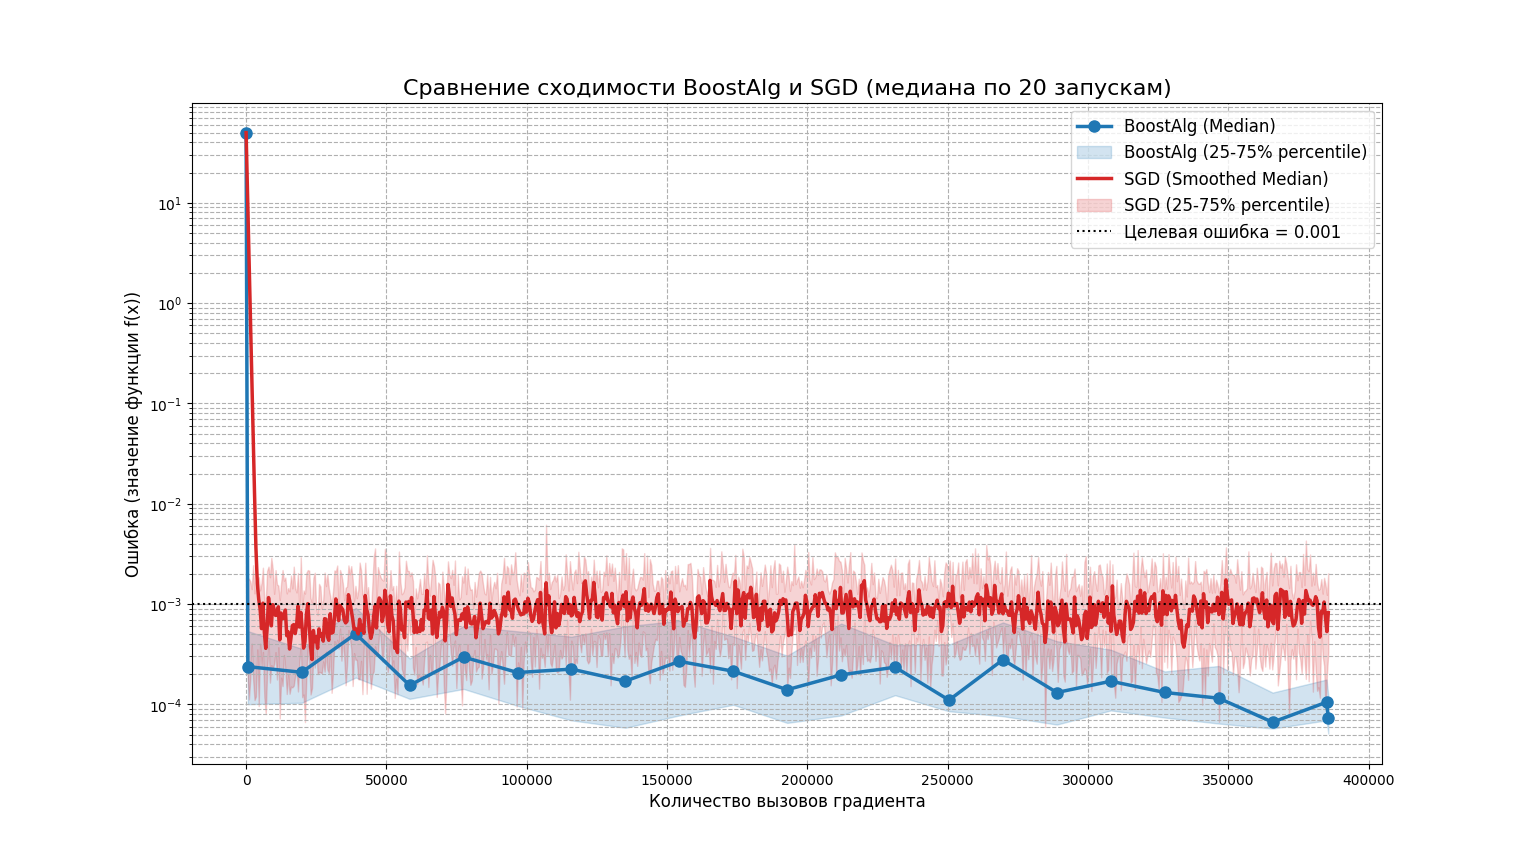
\includegraphics[width=\textwidth]{SGD_vs_BoostAlg.png}
\caption{График сходимости: ошибка $f(x) - f^*$ от количества вызовов оракула. Сплошная линия — медиана, закрашенная область — разброс между 0.25 и 0.75 квантилями.}
\label{fig:convergence}
\end{figure}

\subsection{Выводы}

Эксперимент подтверждает теоретические преимущества \texttt{BoostAlg}:
\begin{itemize}
    \item \textbf{Высокая надежность}: \texttt{BoostAlg} достиг целевой точности во всех запусках, что соответствует теоретической гарантии ($p < 0.05$).
    \item \textbf{Ненадежность SGD}: При том же бюджете \texttt{SGD} потерпел неудачу почти в половине случаев (35\%).
    \item \textbf{Цена надежности}: Более медленная начальная сходимость \texttt{BoostAlg} является платой за внутренние процедуры, которые гарантируют достижение результата.
\end{itemize}
Таким образом, \texttt{BoostAlg} является эффективным инструментом для задач стохастической оптимизации, где требуется высокая и предсказуемая вероятность успеха.

\section{Заключение}

В настоящей дипломной работе были исследованы и разработаны методы для решения задач стохастической выпуклой оптимизации и седловых задач, обеспечивающие сходимость с высокой вероятностью. В отличие от классических подходов, гарантирующих сходимость лишь по математическому ожиданию, предложенные алгоритмы позволяют получить решение заданной точности $\epsilon$ с вероятностью не менее $1-p$ при малых $p$.

На защиту выносятся следующие основные результаты:

\begin{enumerate}
    \item \textbf{Обобщенный мета-алгоритм для сходимости с высокой вероятностью.} Разработана и теоретически обоснована модификация алгоритма \texttt{proxBoost} для широкого класса задач выпуклой оптимизации, включая негладкие и не сильно выпуклые случаи. Данный подход представляет собой универсальную <<обертку>>, позволяющую преобразовать любой алгоритм со сходимостью по математическому ожиданию в алгоритм со сходимостью с высокой вероятностью. При этом оракульная сложность возрастает лишь логарифмически по $1/p$.

    \item \textbf{Новые оценки оракульной сложности.} Получены детальные оценки сложности для разработанного мета-алгоритма в следующих классах задач:
    \begin{itemize}
        \item сильно выпуклые негладкие функции;
        \item выпуклые гладкие функции;
        \item выпуклые негладкие функции.
    \end{itemize}
    Показано, что итоговая сложность имеет слабую (логарифмическую) зависимость от вероятности  $p$ и близкую к оптимальной зависимость от точности $\epsilon$.

    \item \textbf{Применимость подхода к седловым задачам.} Продемонстрирована универсальность лежащих в основе метода идей (неточный проксимальный метод и робастная оценка расстояний) путем их применения для решения стохастических выпукло-вогнутых седловых задач, что подтверждает общность и фундаментальность подхода.

    \item \textbf{Экспериментальное подтверждение надежности.} Результаты вычислительного эксперимента наглядно демонстрируют теоретические преимущества предложенного подхода. В условиях плохо обусловленной задачи алгоритм \texttt{BoostAlg} обеспечивает гарантированную сходимость при том же бюджете вызовов оракула, при котором стандартный \texttt{SGD} показывает крайне низкую надежность.
\end{enumerate}

Таким образом, в работе представлен комплексный подход к построению надежных и эффективных алгоритмов стохастической оптимизации, подкрепленный теоретическими оценками и практическими результатами.






\printbibliography[heading=bibintoc]
	
\end{document}
